\documentclass[11pt]{article}

% ------------------------------------------------------------
% Packages
% ------------------------------------------------------------
\usepackage[margin=1in]{geometry}
\usepackage{amsmath, amssymb, amsfonts, mathtools}
\usepackage{graphicx}
\usepackage{booktabs}
\usepackage{multirow}
\usepackage{array}
\usepackage{xcolor}
\usepackage{hyperref}
\usepackage{caption}
\usepackage{subcaption}
\usepackage{enumitem}
\usepackage{microtype}

% ------------------------------------------------------------
% Hyperref setup
% ------------------------------------------------------------
\hypersetup{
    colorlinks=true,
    linkcolor=blue!50!black,
    citecolor=blue!50!black,
    urlcolor=blue!50!black
}

% ------------------------------------------------------------
% Macros
% ------------------------------------------------------------
\newcommand{\R}{\mathbb{R}}
\newcommand{\E}{\mathbb{E}}
\newcommand{\KL}{\mathrm{KL}}
\newcommand{\softmax}{\mathrm{softmax}}
\newcommand{\TopK}{\mathrm{TopK}}
\newcommand{\argmin}{\operatorname*{arg\,min}}
\newcommand{\norm}[1]{\left\lVert #1 \right\rVert}

\newcommand{\teacher}{T}
\newcommand{\student}{S}

% ------------------------------------------------------------
% Title
% ------------------------------------------------------------
\title{
    Compressing World Models for Planning:\\
    Activation-Aware Low-Rank Approximation and the Fragility of Operator Distillation
}

\author{
    Daniel Enriquez \\
    NYU Tandon School of Engineering \\
    \texttt{[email]}
}

\date{}

\begin{document}

\maketitle

% ------------------------------------------------------------
% Abstract
% ------------------------------------------------------------
\begin{abstract}
World models are increasingly used as predictive components inside planning systems, but their computational cost can make deployment expensive. 
This paper studies post-training compression of world models for closed-loop model-predictive control. 
We compare weight-based low-rank compression, activation-aware low-rank compression, and cache-based operator distillation objectives that attempt to preserve the planner-facing cost function induced by the model.
Across TwoRoom and PushT environments using LeWM checkpoints, we find that activation-aware SVD is a strong and stable baseline, while naive operator-aware fine-tuning is fragile and can underperform the compressed model before fine-tuning.
Our results suggest that preserving predictor activations may be more reliable than matching teacher costs over uniformly sampled candidate trajectories, and that effective operator-aware compression likely requires supervision aligned with the planner's elite action distribution.
\end{abstract}

% ------------------------------------------------------------
% 1. Introduction
% ------------------------------------------------------------
\section{Introduction}

World models are attractive because they let an agent reason about the consequences of actions before taking them. Instead of learning a direct policy, a world-model-based planner evaluates many candidate action sequences under a learned predictive model and selects actions through model-predictive control. This design is useful because the learned model can, in principle, be reused across goals, planning horizons, and downstream control procedures. However, it also makes inference expensive: every environment step may require hundreds of model evaluations inside a planner such as the cross-entropy method (CEM). As world models become larger and more capable, reducing their computational and memory cost becomes important for deployment.

Compression for world models is not identical to compression for ordinary supervised predictors. In image classification, a compressed model is usually evaluated by whether it preserves top-1 accuracy or logits on a fixed input distribution. In planning, the model is embedded inside a decision-making loop. Small distortions in predicted costs can change the ranking of candidate action sequences, which can then change the selected action and compound over time through closed-loop interaction. Therefore, a compressed world model should not only preserve weights, activations, or one-step prediction quality; it should preserve the planner-facing behavior induced by the model.

This paper studies post-training compression of learned world models used for closed-loop model-predictive control. We focus on LeWM-style world models in TwoRoom and PushT, where a pretrained teacher model evaluates candidate action sequences and a CEM-based planner selects actions. We compress the model's predictor components using low-rank approximations and evaluate the resulting models by closed-loop MPC success rate. Our central question is:

\[
    \textit{Can we compress a world model while preserving the closed-loop behavior of the planner that uses it?}
\]

We compare three families of methods. First, we use a simple weight-space low-rank baseline, which applies SVD directly to predictor weight matrices. Second, we use activation-aware SVD, which chooses low-rank approximations that better preserve predictor outputs on calibration activations. Third, we test operator-aware distillation objectives. These objectives are motivated by the fact that the planner interacts with the world model through a cost operator over candidate action sequences. Instead of only preserving internal activations, operator-aware distillation attempts to fine-tune the compressed model so that its candidate-action costs match those of the teacher.

Our operator-aware methods use a cached teacher-cost dataset. For each sampled state-goal pair, we uniformly sample candidate action sequences, evaluate their costs under the teacher, and store the resulting cost table. The compressed student is then fine-tuned without further teacher rollouts. We test a forward-KL objective over teacher and student cost-induced distributions, as well as a hybrid objective that combines this KL term with an elite-candidate classification loss. This setup is deliberately lightweight: it reuses the existing planner-facing cost interface, avoids expensive online teacher calls during distillation, and fits naturally into a post-training compression workflow.

The empirical results are mixed in an informative way. Activation-aware SVD is a strong and stable baseline, especially on TwoRoom, where it preserves closed-loop success even under substantial predictor compression. On PushT, compression is more damaging, but the simple low-rank baselines still often outperform the operator-aware fine-tuned models. The operator-aware objectives are inconsistent: in some aggressive-compression settings they recover performance relative to the corresponding compressed initialization, but in many cases they degrade closed-loop success. This suggests that naively matching cached teacher costs is not sufficient to preserve planner behavior.

We interpret this fragility as a mismatch between the offline operator-distillation signal and the distribution that matters during planning. The current cache uses uniformly sampled action sequences, while CEM planning concentrates on elite or near-elite regions of action space. A KL loss over uniformly sampled candidates can spend gradient matching irrelevant ``junk-versus-junk'' rankings rather than preserving the few distinctions that determine the planner's selected action. Similarly, top-\(k\) elite labels can be unstable when many candidates have near-tied teacher costs. Thus, operator-aware compression is a plausible direction, but the supervision must be aligned with the planner's actual candidate distribution.

Our contributions are as follows:

\begin{enumerate}[leftmargin=*]
    \item We evaluate post-training low-rank compression of world models under closed-loop MPC, rather than relying only on offline reconstruction or distillation losses.
    \item We compare weight SVD, activation-aware SVD, and cache-based operator-aware distillation across TwoRoom and PushT using LeWM teacher checkpoints.
    \item We show that activation-aware SVD is a strong baseline for world-model compression, often preserving closed-loop success better than naive operator fine-tuning.
    \item We identify a failure mode of cache-only operator distillation: matching teacher costs over uniformly sampled candidates can be misaligned with CEM planning behavior.
    \item We argue that future operator-aware compression methods should use planner-aligned candidate distributions, such as CEM-refined candidates, top-\(k\)-restricted objectives, or preference losses focused on elite action regions.
\end{enumerate}

Overall, the lesson is not that operator-aware compression is ineffective, but that the naive version is fragile. Closed-loop planning exposes errors that offline losses may hide. For world models, compression should be judged by the behavior of the full planning system, and operator-aware objectives should be designed around the action distributions that the planner actually uses.
% Motivation:
% - World models are useful for planning but computationally expensive.
% - Compression matters for deployment and repeated planning.
% - Unlike standard supervised models, world models are used inside planners.
% - Therefore, compression should be evaluated by closed-loop control performance,
%   not only by reconstruction/prediction error.

% Main question:
% Can we compress a world model while preserving its closed-loop planning behavior?

% Initial hypothesis:
% Since the world model induces a cost over candidate action sequences, perhaps
% compression should preserve this operator, not merely weights or activations.

% Summary of approach:
% - Compress predictor layers with Weight SVD and Activation-aware SVD.
% - Fine-tune compressed models using cached teacher operator costs.
% - Evaluate via closed-loop MPC success on TwoRoom and PushT.

% Main finding:
% Activation-aware SVD is surprisingly strong.
% Operator-aware fine-tuning is inconsistent and often fragile.

% Contributions:
% 1. A closed-loop evaluation protocol for compressed world models.
% 2. A comparison of weight SVD, activation-aware SVD, and operator-aware distillation.
% 3. Empirical evidence that naive cache-only operator distillation can hurt performance.
% 4. Analysis of why uniformly sampled candidate-action supervision may be misaligned
%    with planner behavior.

% ------------------------------------------------------------
% 2. Background
% ------------------------------------------------------------
\section{Background}

\subsection{World Models for Planning}

A world model is a learned approximation of environment dynamics that allows an agent to reason about the consequences of actions before executing them. In the model-based reinforcement learning literature, this idea is often described as learning an internal simulator or ``imagination'' model: given observations and actions, the model learns a compact representation of the environment and predicts how that representation evolves over time. Ha and Schmidhuber's recurrent world model is a canonical example: the model learns compressed spatio-temporal representations of an environment, and policies can then be trained or evaluated using features produced by the learned model rather than directly from raw observations \citep{ha2018worldmodels}. This line of work motivates our setting: the model is not merely a passive predictor, but a component used by a downstream decision procedure.

In planning-based control, the world model remains active at inference time. Given a current observation $o_t$ and a candidate action sequence
\[
    a_{t:t+H-1} = (a_t, a_{t+1}, \dots, a_{t+H-1}),
\]
the model predicts future latent states or observations and assigns a cost to the resulting imagined trajectory. A planner then searches over action sequences and selects the one with lowest predicted cost. In a goal-conditioned setting, this cost often measures the distance between the predicted final latent state and a goal representation. Abstractly, if $f_\theta$ denotes the learned latent dynamics model, the rollout is
\[
    \hat z_{t+1} = f_\theta(\hat z_t, a_t),
    \qquad
    \hat z_t = e_\theta(o_t),
\]
and a terminal goal-matching cost can be written as
\[
    C_\theta(a_{t:t+H-1}; o_t, o_g)
    =
    \left\lVert \hat z_{t+H} - z_g \right\rVert_2^2,
    \qquad
    z_g = e_\theta(o_g).
\]
The planner approximately solves
\[
    a_{t:t+H-1}^\star
    =
    \arg\min_{a_{t:t+H-1}}
    C_\theta(a_{t:t+H-1}; o_t, o_g).
\]
In practice, this optimization is usually solved approximately by a sampling-based optimizer such as the Cross-Entropy Method (CEM), which repeatedly samples candidate action sequences, evaluates their predicted costs under the world model, keeps the lowest-cost candidates as elites, and updates the sampling distribution toward those elites.

This makes world-model compression different from ordinary predictor compression. For a classifier, preserving logits or accuracy on a fixed validation set may be sufficient. For a planning world model, the compressed model must preserve the induced ordering of candidate action sequences, especially near the elite region used by the planner. A small distortion in predicted costs may not matter if it leaves the best candidates unchanged, but a similarly small distortion can be harmful if it changes which candidate sequence CEM selects. Thus, the object being compressed is not only a neural network function, but the cost operator exposed to the planner.

Our experiments use LeWorldModel (LeWM), a recent latent world model based on a Joint Embedding Predictive Architecture (JEPA). LeWM learns an encoder that maps raw pixel observations into compact latent embeddings and a predictor that models action-conditioned dynamics in this latent space. Unlike reconstruction-based world models, LeWM is trained to predict future embeddings rather than pixels. The model uses two loss terms: a next-embedding prediction loss and a SIGReg regularizer that encourages the latent embedding distribution to match an isotropic Gaussian, preventing representational collapse without stop-gradient, exponential moving averages, or a frozen pretrained encoder \citep{maes2026leworldmodel}. The reported LeWM model has roughly $15$M parameters, trains on a single GPU, and is designed for efficient latent planning; the paper reports planning speedups of up to $48\times$ relative to foundation-model-based world models while remaining competitive on several control tasks \citep{maes2026leworldmodel}.

At inference time, LeWM performs latent-space model-predictive control. The current observation and goal observation are encoded into latent vectors, the predictor rolls candidate action sequences forward in latent space, and CEM optimizes a latent terminal cost. The first action, or a short prefix of the optimized sequence, is executed before replanning from the next observation. This receding-horizon structure is important for our work: even though the world model is fixed during evaluation, it is queried many times inside each planning step. Therefore, reducing predictor size can reduce the cost of each candidate rollout, but any compression error is repeatedly amplified through the planner's candidate evaluation and action-selection loop.

This paper studies exactly that regime. We do not retrain LeWM from scratch or change its planning semantics. Instead, we take pretrained LeWM checkpoints and compress the predictor components used during latent rollout. The resulting model is evaluated through the same closed-loop MPC procedure as the teacher. This lets us ask whether low-rank compression preserves the planner-facing behavior of the world model, rather than only preserving internal activations or offline prediction losses.

\subsection{Compression of Neural Predictors}

Modern neural networks often contain substantial redundancy in their learned parameterization. A common way to exploit this redundancy is to replace dense weight matrices with lower-rank approximations. Given a linear layer with weight matrix
\[
    W \in \mathbb{R}^{d_{\mathrm{in}} \times d_{\mathrm{out}}},
\]
standard low-rank compression approximates $W$ by a rank-$r$ factorization
\[
    W \approx U_r V_r,
    \qquad
    U_r \in \mathbb{R}^{d_{\mathrm{in}} \times r},
    \qquad
    V_r \in \mathbb{R}^{r \times d_{\mathrm{out}}},
\]
typically obtained from a truncated singular value decomposition. When $r \ll \min(d_{\mathrm{in}}, d_{\mathrm{out}})$, this reduces the number of parameters and matrix multiplication cost from $d_{\mathrm{in}}d_{\mathrm{out}}$ to
\[
    r(d_{\mathrm{in}} + d_{\mathrm{out}}).
\]
This approach is attractive because it is simple, architecture-agnostic, and can be applied post hoc to pretrained models without access to the original training procedure.

However, ordinary weight-space low-rank approximation is not necessarily aligned with model behavior. Minimizing
\[
    \lVert W - U_r V_r \rVert_F^2
\]
preserves the weight matrix in Frobenius norm, but the downstream computation depends on the distribution of layer inputs. If a layer is usually evaluated on activations $X \in \mathbb{R}^{n \times d_{\mathrm{in}}}$, then the relevant error is closer to
\[
    \lVert XW - XU_rV_r \rVert_F^2.
\]
This motivates activation-aware compression, where the approximation is chosen to preserve the layer's output on representative calibration inputs. In our setting, those calibration inputs are not arbitrary image batches; they arise from world-model cost evaluation under sampled candidate action sequences. This distinction matters because the predictor is used inside a planner, so the relevant activation distribution is induced by latent rollouts and candidate plans.

We therefore compare two direct compression baselines. The first is weight SVD, which compresses predictor weights using only the pretrained parameters. The second is activation-aware SVD, which uses calibration rollouts to find low-rank approximations that better preserve predictor activations on the states and candidate action sequences seen during planning. Both methods are purely structural: they produce compressed predictors without additional task-level fine-tuning. These baselines are important because they separate the effect of simple low-rank redundancy from any additional benefit of operator-aware training.

\subsection{Planner-Facing Distillation}

A world model used for planning exposes more than a one-step prediction function. It induces a cost operator over candidate action sequences. For a state or observation context $s$ and a candidate plan $a_{1:H}^{(i)}$, the world model assigns a scalar cost
\[
    c_\theta(s, a_{1:H}^{(i)}).
\]
A planner such as CEM uses these costs to rank candidate plans and update its sampling distribution. Therefore, for closed-loop control, the most important question is not whether a compressed model exactly matches the teacher's internal activations, but whether it preserves the action-sequence preferences that drive planning.

This motivates an operator-aware view of compression. Let the teacher world model define costs
\[
    c_i^T = c_{\theta_T}(s, a_{1:H}^{(i)})
\]
and let the compressed student define costs
\[
    c_i^S = c_{\theta_S}(s, a_{1:H}^{(i)}).
\]
Rather than distilling predictions in pixel space or latent embedding space, one can distill the planner-facing cost landscape over a finite candidate set
\[
    \{a_{1:H}^{(i)}\}_{i=1}^C.
\]
The hope is that even if the student does not exactly reproduce the teacher's dynamics everywhere, it may still preserve the relative ordering of candidate plans in the regions relevant to CEM.

In our implementation, we build an operator cache by sampling states from the evaluation dataset and sampling candidate action sequences uniformly from the action range. For each state and candidate sequence, we store the teacher cost, the teacher's best candidate, and top-$k$ elite indices. This cache provides a fixed offline supervision signal for distillation. The student is initialized from a compressed predictor and then fine-tuned using only cached teacher costs and reconstructed planning contexts. No simulator rollout, online teacher query, or CEM optimization is performed during distillation. This makes the method lightweight and reproducible, but also limits the quality of the supervision: the cached candidate set is random rather than drawn from the teacher's actual CEM proposal distribution.

\subsection{Cost-Distribution and Elite Distillation Objectives}

A natural way to distill the teacher cost operator is to convert costs into a probability distribution over candidate action sequences. For each state, we normalize costs across candidates, for example by z-scoring,
\[
    \tilde c_i
    =
    \frac{c_i - \mu(c)}{\max(\sigma(c), \epsilon)}.
\]
We then define a Boltzmann distribution over plans:
\[
    p(i \mid s)
    =
    \frac{\exp(-\tilde c_i/\tau)}
    {\sum_{j=1}^C \exp(-\tilde c_j/\tau)}.
\]
Lower-cost plans receive higher probability. Given teacher and student distributions $p_T$ and $p_S$, one possible distillation objective is the forward KL divergence
\[
    \mathcal{L}_{\mathrm{KL}}
    =
    \frac{1}{|B|}
    \sum_{s \in B}
    \mathrm{KL}\!\left(
        p_T(\cdot \mid s)
        \,\Vert\,
        p_S(\cdot \mid s)
    \right).
\]
This encourages the student to assign probability mass wherever the teacher assigns mass. In principle, it preserves the teacher's soft preference distribution over candidate plans.

A second objective focuses only on the teacher's elite set. Let
\[
    E_s = \operatorname{TopK}_{\mathrm{lowest}}\{c_1^T,\dots,c_C^T\}
\]
denote the $k$ candidate plans with lowest teacher cost for state $s$. We form binary labels
\[
    y_i = \mathbf{1}[i \in E_s]
\]
and train the student to assign higher scores to elite candidates using logits
\[
    z_i = -\tilde c_i^S/\tau_{\mathrm{elite}}.
\]
The elite classification loss is a balanced binary cross-entropy over elite and non-elite candidates:
\[
    \mathcal{L}_{\mathrm{elite}}
    =
    \frac{1}{|E_s|}
    \sum_{i \in E_s}
    \operatorname{BCE}(z_i,1)
    +
    \frac{1}{C-|E_s|}
    \sum_{i \notin E_s}
    \operatorname{BCE}(z_i,0).
\]
We also evaluate a hybrid objective,
\[
    \mathcal{L}_{\mathrm{hybrid}}
    =
    \lambda_{\mathrm{KL}}\mathcal{L}_{\mathrm{KL}}
    +
    \lambda_{\mathrm{elite}}\mathcal{L}_{\mathrm{elite}},
\]
which combines soft cost-distribution matching with explicit top-$k$ preservation.

These objectives are reasonable from a planner-aware perspective, but they are not guaranteed to improve closed-loop control. If the candidate set contains mostly uniformly random plans, many comparisons are between poor actions that CEM would never consider after its first few refinement steps. In that case, matching the teacher over the full cached distribution may spend capacity preserving irrelevant parts of the cost landscape. Furthermore, because closed-loop success is discontinuous in the selected action sequence, a lower distillation loss does not necessarily imply better control. Our experiments directly expose this gap: operator-aware fine-tuning can reduce cached training losses while degrading closed-loop success.

\subsection{Positioning of This Work}

Our work is best understood as an empirical study of compression for planner-facing latent world models. We do not propose a new world-model architecture, nor do we retrain LeWM. Instead, we ask whether a pretrained latent world model can be compressed while preserving closed-loop MPC performance. This places our contribution between model compression and model-based control: the compression target is a neural predictor, but the evaluation target is the induced planner behavior.

The central observation is that low-rank compression can preserve closed-loop performance surprisingly well, especially at moderate compression levels, but operator-aware fine-tuning is fragile under a simple cache-only protocol. On TwoRoom, several compressed models match or slightly exceed the teacher within the noise of $n=64$ evaluation episodes. On PushT, the teacher remains substantially stronger, but low-rank compression still preserves nontrivial control performance across a range of predictor compression ratios. In contrast, the current operator-cost and hybrid distillation objectives often fail to improve over their compressed initializations and sometimes perform worse.

This negative result is informative. It suggests that planner-aware distillation requires more care than simply matching cached teacher costs over uniformly sampled candidate plans. A stronger method may need candidate distributions closer to the planner's own search distribution, held-out operator caches, lower learning rates, early stopping tied to closed-loop validation, pairwise preference objectives, or direct preservation of CEM elite rankings. We therefore frame the operator-aware methods in this paper as diagnostic baselines rather than as the final solution. The positive result is that simple low-rank predictor compression already gives a useful frontier; the cautionary result is that post-compression operator fine-tuning can easily damage the cost geometry used by MPC.

% Define world model in this context.
% The model predicts or scores future trajectories conditioned on current state,
% goal, and candidate action sequence.
% In LeWM-style planning, the model is used by MPC/CEM to evaluate candidate actions.


\section{Method}
\label{sec:method}

We study post-training compression for latent world models used inside model predictive control. Our goal is not to train a new world model from scratch, but to take a pretrained LeWM model and reduce the size of its predictor while preserving closed-loop planning performance. This distinction is important: because the world model remains inside the control loop at inference time, compression quality must be measured by the behavior of the induced planner, not only by reconstruction error, parameter count, or offline loss.

\subsection{Problem Setup}
\label{sec:problem_setup}

Let a pretrained latent world model consist of an encoder $e_\theta$ and a predictor $f_\phi$. Given an observation $o_t$, the encoder produces a latent state
\[
    z_t = e_\theta(o_t).
\]
Given a latent state and an action sequence $a_{t:t+H-1}$, the predictor rolls the latent state forward for $H$ steps:
\[
    \hat z_{t+h+1}
    =
    f_\phi(\hat z_{t+h}, a_{t+h}),
    \qquad
    \hat z_t = z_t.
\]
For goal-conditioned planning, the goal observation $o_g$ is encoded as
\[
    z_g = e_\theta(o_g),
\]
and the terminal latent planning cost is computed as
\[
    C_\phi(o_t, o_g, a_{t:t+H-1})
    =
    \left\lVert \hat z_{t+H} - z_g \right\rVert_2^2.
\]
At evaluation time, a sampling-based planner uses this cost to choose actions. In our experiments, planning is performed by the Cross-Entropy Method (CEM). CEM samples candidate action sequences, evaluates their costs under the world model, selects low-cost elite plans, and updates its proposal distribution. This process is repeated for a fixed number of iterations, after which the selected action sequence is executed in a receding-horizon MPC loop.

We denote the original pretrained model as the teacher, with predictor parameters $\phi_T$, and a compressed model as the student, with predictor parameters $\phi_S$. The compression problem is to construct $\phi_S$ such that the student has fewer predictor parameters than the teacher while preserving the closed-loop success rate of the MPC controller induced by the model:
\[
    \mathrm{MPC}(e_\theta, f_{\phi_S})
    \approx
    \mathrm{MPC}(e_\theta, f_{\phi_T}).
\]
We keep the encoder fixed and only compress the predictor. This isolates the effect of dynamics-model compression and avoids changing the representation space in which planning costs are computed.

\subsection{Low-Rank Predictor Compression}
\label{sec:low_rank_compression}

The LeWM predictor contains a large fraction of the model's parameters. We therefore target predictor modules for compression while leaving the encoder and other non-predictor components unchanged. For each selected linear layer with weight matrix
\[
    W \in \mathbb{R}^{d_{\mathrm{in}} \times d_{\mathrm{out}}},
\]
we replace $W$ by a low-rank factorization
\[
    W \approx U_r V_r,
\]
where
\[
    U_r \in \mathbb{R}^{d_{\mathrm{in}} \times r},
    \qquad
    V_r \in \mathbb{R}^{r \times d_{\mathrm{out}}}.
\]
The rank $r$ is chosen as a fraction of the maximum possible rank:
\[
    r = \left\lfloor \rho \cdot \min(d_{\mathrm{in}}, d_{\mathrm{out}}) \right\rfloor,
\]
where $\rho \in (0,1]$ is the rank fraction. We evaluate rank fractions
\[
    \rho \in \{0.9, 0.8, 0.7, 0.6, 0.5\}.
\]

We report two compression ratios. The predictor compression ratio is
\[
    \mathrm{CR}_{\mathrm{pred}}
    =
    \frac{\#\mathrm{params}(f_{\phi_S})}
    {\#\mathrm{params}(f_{\phi_T})},
\]
and the total compression ratio is
\[
    \mathrm{CR}_{\mathrm{total}}
    =
    \frac{\#\mathrm{params}(e_\theta, f_{\phi_S})}
    {\#\mathrm{params}(e_\theta, f_{\phi_T})}.
\]
Since the encoder remains fixed, the total compression ratio is less aggressive than the predictor compression ratio. This distinction matters because the practical memory savings are determined by the full model, while our intervention is localized to the predictor.

\paragraph{Weight-SVD compression.}
The simplest baseline applies truncated SVD directly to each target weight matrix:
\[
    W = U \Sigma V^\top,
\]
and retains the top $r$ singular directions:
\[
    W_r = U_{:,:r}\Sigma_{:r,:r}V_{:,:r}^\top.
\]
The dense linear map is then replaced by two consecutive linear maps implementing this rank-$r$ approximation. This method does not require calibration data and serves as a purely parameter-space compression baseline.

\paragraph{Activation-aware SVD compression.}
Weight-space approximation may preserve the matrix $W$ without preserving the layer's output on the inputs that actually occur during planning. We therefore also evaluate activation-aware SVD. Let
\[
    X \in \mathbb{R}^{n \times d_{\mathrm{in}}}
\]
denote a matrix of calibration activations collected from predictor calls under sampled states and candidate action sequences. Instead of minimizing $\lVert W - W_r \rVert_F^2$, activation-aware compression aims to minimize
\[
    \lVert XW - XW_r \rVert_F^2.
\]
This objective better reflects the predictor's behavior under the activation distribution induced by latent rollouts. In our implementation, calibration examples are obtained from the same world-model planning pathway used during evaluation: states and candidate action sequences are passed through the predictor, and layer inputs are recorded for the target modules. The resulting low-rank approximation is then installed in the model and evaluated in closed loop.

\subsection{Operator Cache Construction}
\label{sec:operator_cache}

Low-rank compression is a structural intervention. To test whether post-compression fine-tuning can recover planner-relevant behavior, we construct an offline operator cache from the teacher model. The cache stores the teacher's cost values over sampled states and candidate action sequences.

For each sampled state-goal context $s_j$, we sample $C$ candidate action sequences
\[
    A_j =
    \{a_{j,1:H}^{(1)}, \dots, a_{j,1:H}^{(C)}\},
\]
with actions sampled uniformly from the environment's action range. The teacher assigns each candidate a scalar planning cost:
\[
    c_{j,i}^{T}
    =
    C_{\phi_T}(s_j, a_{j,1:H}^{(i)}).
\]
The cache stores the candidate action tensor
\[
    A \in \mathbb{R}^{S \times C \times H \times d_a},
\]
the teacher cost tensor
\[
    C^T \in \mathbb{R}^{S \times C},
\]
and the teacher's top-$k$ candidate indices for each state:
\[
    E_j^{(k)}
    =
    \operatorname{TopK}_{\mathrm{lowest}}
    \{c_{j,1}^{T}, \dots, c_{j,C}^{T}\}.
\]
In our experiments, the main operator cache contains
\[
    S = 512
\]
states and
\[
    C = 128
\]
candidate action sequences per state, with planning horizon
\[
    H = 5.
\]

The operator cache is used only during distillation. It is not used during closed-loop evaluation. During evaluation, each compressed model is placed inside the original CEM/MPC loop and tested directly in the environment.

\subsection{Operator-Aware Distillation}
\label{sec:operator_distillation}

After low-rank compression, we optionally fine-tune the student predictor using the cached teacher costs. The teacher is not queried online during this stage. For each training step, we sample a minibatch of states and candidate action sequences from the operator cache. The student computes costs for the same state-candidate pairs:
\[
    c_{j,i}^{S}
    =
    C_{\phi_S}(s_j, a_{j,1:H}^{(i)}).
\]
Only predictor parameters are trainable; all non-predictor parameters are frozen. This preserves the encoder representation and restricts fine-tuning to the compressed dynamics model.

\paragraph{Cost-distribution KL.}
The first objective matches the teacher and student cost distributions over candidates. For each state, teacher and student costs are normalized across candidates:
\[
    \tilde c_{j,i}^{T}
    =
    \frac{c_{j,i}^{T} - \mu(c_j^T)}
    {\max(\sigma(c_j^T), \epsilon)},
    \qquad
    \tilde c_{j,i}^{S}
    =
    \frac{c_{j,i}^{S} - \mu(c_j^S)}
    {\max(\sigma(c_j^S), \epsilon)}.
\]
We convert normalized costs into Boltzmann distributions:
\[
    p_T(i \mid s_j)
    =
    \frac{\exp(-\tilde c_{j,i}^{T}/\tau)}
    {\sum_{\ell=1}^{C}\exp(-\tilde c_{j,\ell}^{T}/\tau)},
\]
\[
    p_S(i \mid s_j)
    =
    \frac{\exp(-\tilde c_{j,i}^{S}/\tau)}
    {\sum_{\ell=1}^{C}\exp(-\tilde c_{j,\ell}^{S}/\tau)}.
\]
The cost-KL objective is
\[
    \mathcal{L}_{\mathrm{KL}}
    =
    \frac{1}{|B|}
    \sum_{j \in B}
    \mathrm{KL}
    \left(
        p_T(\cdot \mid s_j)
        \,\Vert\,
        p_S(\cdot \mid s_j)
    \right).
\]
This loss encourages the student to preserve the teacher's soft preference distribution over candidate plans.

\paragraph{Elite classification.}
The second objective focuses on the teacher's elite candidates. For each state $s_j$, let $E_j$ denote the indices of the $k$ lowest-cost teacher candidates. We define binary labels
\[
    y_{j,i}
    =
    \mathbf{1}[i \in E_j].
\]
The student logits are negative normalized costs:
\[
    z_{j,i}
    =
    -\tilde c_{j,i}^{S}/\tau_{\mathrm{elite}}.
\]
We train the student with a balanced binary cross-entropy:
\[
    \mathcal{L}_{\mathrm{elite}}
    =
    \frac{1}{|B|}
    \sum_{j \in B}
    \left[
    \frac{1}{|E_j|}
    \sum_{i \in E_j}
    \operatorname{BCE}(z_{j,i},1)
    +
    \frac{1}{C-|E_j|}
    \sum_{i \notin E_j}
    \operatorname{BCE}(z_{j,i},0)
    \right].
\]
This objective directly encourages the student to assign lower costs to teacher-preferred plans.

\paragraph{Hybrid objective.}
We also evaluate a hybrid objective combining the two signals:
\[
    \mathcal{L}_{\mathrm{hybrid}}
    =
    \lambda_{\mathrm{KL}}\mathcal{L}_{\mathrm{KL}}
    +
    \lambda_{\mathrm{elite}}\mathcal{L}_{\mathrm{elite}}.
\]
In our experiments, we use
\[
    \lambda_{\mathrm{KL}} = 1,
    \qquad
    \lambda_{\mathrm{elite}} = 1,
\]
unless otherwise specified.

\subsection{Evaluation Protocol}
\label{sec:evaluation_protocol}

The primary metric is closed-loop MPC success rate. Each model is evaluated by replacing the teacher predictor with the compressed or distilled predictor inside the same planning loop. The planner, environment, evaluation dataset, goal sampling protocol, and random seed are held fixed within each environment. This ensures that differences in success rate are attributable to the compressed model rather than to changes in the controller.

For each environment, we evaluate the teacher, weight-SVD baselines, activation-aware SVD baselines, and operator-aware distilled models. All reported preliminary results use
\[
    n = 64
\]
evaluation episodes with seed $0$. Therefore, one successful episode corresponds to
\[
    \frac{1}{64} \times 100 = 1.5625
\]
percentage points. We treat small differences at this scale cautiously and emphasize trends across compression ratios rather than single-point improvements.

We report success rate as a function of total compression ratio and predictor compression ratio. The total compression ratio measures full-model parameter reduction, while predictor compression ratio isolates the part of the model actually compressed. This gives two complementary views of the compression frontier: practical model-size reduction and predictor-specific compression strength.

\subsection{Why Operator-Aware Distillation Is Natural but Fragile}
\label{sec:operator_distillation_fragility}

The motivation for operator-aware distillation is straightforward. In latent world models used for planning, the predictor is not merely a feature-producing module; it is repeatedly queried inside an optimization procedure. At test time, the model is used to evaluate candidate action sequences, rank them by predicted latent cost, and guide a planner toward actions that reach the goal. Therefore, a compressed world model should ideally preserve not only the original weights or intermediate activations, but also the induced planning operator.

This motivates our operator-aware distillation objective. Given a teacher world model and a compressed student initialized from a low-rank approximation, we build a cache of states, candidate action sequences, and teacher costs. The student is then fine-tuned so that its cost evaluations match the teacher's evaluations on the same candidate plans. Conceptually, this is closer to the downstream use of the model than ordinary weight reconstruction:
\[
    C_{\phi_T}(s,a_{1:H})
    \approx
    C_{\phi_S}(s,a_{1:H}),
\]
where \(C_{\phi_T}\) and \(C_{\phi_S}\) denote the teacher and student planning costs induced by latent rollouts. If successful, such a procedure should preserve the part of the world model that matters most for model-predictive control: the ability to score and rank candidate action sequences.

However, our preliminary results suggest that this idea is more delicate than the motivation alone would imply. In our experiments, operator-aware fine-tuning sometimes improved aggressive compression settings, but it also sometimes degraded performance relative to the corresponding SVD initialization. We do not interpret this as evidence against operator-aware compression in general. Rather, it indicates that the particular cache-only distillation objectives tested here are not yet reliably aligned with closed-loop planning performance.

One source of fragility is the mismatch between the distillation cache and the planner's actual query distribution. Our current cache samples candidate action sequences uniformly from the action range:
\[
    a_{1:H}^{(i)} \sim \mathrm{Unif}([-1,1]^{H \times d_a}).
\]
During evaluation, by contrast, CEM iteratively concentrates its samples around low-cost regions. The planner's decisions are therefore determined by fine distinctions among near-elite candidates, while the distillation objective also spends capacity matching costs on many uniformly sampled candidates that may be irrelevant to the final action choice. As a result, a student may improve its offline cost-matching objective without improving, and sometimes while harming, the action rankings that matter in closed-loop control.

A second source of fragility is that planning is sensitive to local rankings rather than global cost accuracy. The planner ultimately uses the model through an approximately argmin-like operation:
\[
    a^*_{1:H}
    =
    \arg\min_{a_{1:H}} C_\phi(s,a_{1:H}).
\]
Thus, preserving the full teacher cost distribution is not necessarily equivalent to preserving the selected action. A small perturbation to the costs near the optimum can change the elite set selected by CEM, even if the average cost-matching loss remains low. Conversely, a model with imperfect global cost matching may still plan well if it preserves the ordering of the best candidates.

A third issue is that scalar operator losses do not directly constrain the geometry of latent rollouts. The planner evaluates an action sequence by autoregressively rolling out the compressed predictor:
\[
    \hat z_{t+h+1}^{S}
    =
    f_{\phi_S}(\hat z_{t+h}^{S}, a_{t+h}),
    \qquad
    h=0,\dots,H-1.
\]
Fine-tuning only on terminal scalar costs may alter intermediate latent trajectories in ways that are not visible to the cached loss but still affect planning when the model is placed back inside the CEM loop. In this sense, operator distillation is closer to behavioral fine-tuning of a planner than to ordinary reconstruction, and it may require a more carefully matched training distribution.

These limitations should be interpreted in light of the limited scope of our experiments. We only tested a small set of operator-aware objectives, used a fixed cache size, relied primarily on uniformly sampled candidate sequences, and performed limited hyperparameter tuning. The negative or mixed results therefore do not rule out operator-aware distillation. Instead, they identify a specific failure mode of a simple implementation: naively matching cached teacher costs is not guaranteed to improve the closed-loop behavior of a compressed world model.

Overall, operator-aware distillation remains a principled direction for world model compression. The key lesson from our experiments is that the operator objective must be carefully aligned with the planner. Future variants should use planner-matched candidate generation, such as CEM-refined candidates; held-out operator caches; losses focused on near-elite candidates; preference or ranking objectives; and possibly auxiliary constraints on latent rollout geometry. Our results suggest that preserving the planning operator is the right target, but that doing so reliably requires more than a generic cache-only cost-matching loss.

% ------------------------------------------------------------
% 5. Experimental Protocol
% ------------------------------------------------------------
\section{Experimental Protocol}
\label{sec:experimental_protocol}

We evaluate compressed latent world models in the setting that matters for their downstream use: closed-loop planning. Rather than reporting only reconstruction error, parameter count, or offline cost-matching losses, we benchmark each compressed model inside the same model-predictive control pipeline used by the original LeWM checkpoints. This section describes the environments, compression sweep, operator-cache construction, distillation procedure, and closed-loop evaluation protocol.

\subsection{Environments and Models}
\label{sec:envs_models}

We evaluate on two continuous-control environments from the LeWorldModel evaluation suite: \textsc{TwoRoom} and \textsc{PushT}. \textsc{TwoRoom} is a low-dimensional navigation task in which an agent must move between two rooms through a doorway to reach a goal location. \textsc{PushT} is a 2D manipulation task in which an agent must push a T-shaped object toward a target configuration. These environments differ in both visual and control complexity: \textsc{TwoRoom} is a simpler navigation domain, while \textsc{PushT} requires contact-rich manipulation and more precise planning.

For each environment, we use the publicly released LeWM teacher checkpoint:
\[
    \texttt{quentinll/lewm-tworooms}
    \qquad\text{and}\qquad
    \texttt{quentinll/lewm-pusht}.
\]
Both models have approximately \(18.0\) million parameters in total, of which approximately \(10.8\) million belong to the predictor. Since the predictor is the component repeatedly queried during planning rollouts, we focus compression on predictor modules while leaving the rest of the model unchanged. This isolates the effect of compressing the planning-relevant dynamics module.

\subsection{Compression Sweep}
\label{sec:compression_sweep}

We evaluate compression across five rank fractions:
\[
    r \in \{0.9, 0.8, 0.7, 0.6, 0.5\}.
\]
For each rank fraction, we construct compressed models using two direct low-rank baselines: weight-space SVD and activation-aware SVD. Weight-space SVD approximates selected predictor weight matrices directly, while activation-aware SVD uses calibration rollouts to approximate the predictor under the activation distribution induced by the world model evaluation pipeline.

For every compressed model, we report both the total compression ratio and the predictor compression ratio:
\[
    \rho_{\mathrm{total}}
    =
    \frac{\#\text{parameters in compressed model}}
         {\#\text{parameters in teacher model}},
    \qquad
    \rho_{\mathrm{pred}}
    =
    \frac{\#\text{compressed predictor parameters}}
         {\#\text{teacher predictor parameters}}.
\]
The total compression ratio is smaller in magnitude than the predictor compression ratio because only the predictor is compressed; the encoder and other non-predictor components are kept fixed. We then evaluate each compressed model using closed-loop MPC success rate.

\subsection{Operator Cache Construction}
\label{sec:operator_cache}

For operator-aware distillation, we construct an offline cache of teacher planning costs. The cache contains \(S=512\) states per environment. For each cached state, we sample \(C=128\) candidate action sequences of horizon \(H=5\). Candidate actions are sampled uniformly from the action range:
\[
    a_{1:H}^{(i)} \sim \mathrm{Unif}([-1,1]^{H \times d_a}),
    \qquad i=1,\dots,C.
\]
The teacher model evaluates each candidate sequence once, producing a cached cost matrix
\[
    C_T \in \mathbb{R}^{S \times C},
\]
where \(C_T[s,i]\) denotes the teacher cost assigned to candidate \(i\) at cached state \(s\). These costs are computed under \texttt{torch.no\_grad()}, so the teacher is used only to generate fixed supervision targets. The cache also stores the candidate action tensor, top-\(k\) teacher indices, the teacher best candidate index, and the teacher best first action. No online teacher calls, CEM rollouts, or environment interactions are performed during distillation.

This cache design makes the operator-aware methods computationally lightweight: after the cache is built, each distillation step only requires a student cost forward pass on cached states and candidate actions. However, because the candidates are uniformly sampled rather than generated by CEM, the cache distribution does not perfectly match the planner's test-time query distribution. We return to this limitation when interpreting the results.

\subsection{Distillation Setup}
\label{sec:distillation_setup}

Operator-aware methods initialize the student from a compressed checkpoint and then fine-tune the predictor using the cached teacher costs. Unless otherwise stated, distillation is run for \(1000\) gradient steps. Each step samples \(16\) cached states and \(64\) candidate action sequences per state. The optimizer is AdamW with learning rate
\[
    \eta = 10^{-4},
\]
and weight decay set to zero. Only parameters whose names match the predictor substring are trainable; all other parameters are frozen. This ensures that operator-aware fine-tuning only modifies the compressed planning dynamics module rather than changing the entire world model.

We evaluate two main operator-aware objectives. The first is a cost-distribution KL objective, which matches teacher and student softmax distributions over candidate costs. Given normalized teacher and student costs \(\tilde c_T,\tilde c_S \in \mathbb{R}^C\), we define
\[
    p_T(i \mid s)
    =
    \frac{\exp(-\tilde c_T(s,i)/\tau)}
         {\sum_{j=1}^{C}\exp(-\tilde c_T(s,j)/\tau)},
    \qquad
    p_S(i \mid s)
    =
    \frac{\exp(-\tilde c_S(s,i)/\tau)}
         {\sum_{j=1}^{C}\exp(-\tilde c_S(s,j)/\tau)}.
\]
The cost-KL loss is
\[
    \mathcal{L}_{\mathrm{KL}}
    =
    \frac{1}{|B|}
    \sum_{s \in B}
    \mathrm{KL}
    \bigl(
        p_T(\cdot \mid s)
        \,\|\, 
        p_S(\cdot \mid s)
    \bigr).
\]
The second is a hybrid objective that combines this KL term with an elite classification term. The elite labels are obtained from the teacher's lowest-cost candidates. If \(E_s\) denotes the teacher top-\(k\) candidate set for state \(s\), then
\[
    y_i(s) = \mathbf{1}[i \in E_s].
\]
The hybrid objective is
\[
    \mathcal{L}_{\mathrm{hybrid}}
    =
    \lambda_{\mathrm{KL}}\mathcal{L}_{\mathrm{KL}}
    +
    \lambda_{\mathrm{elite}}\mathcal{L}_{\mathrm{elite}}.
\]
In our preliminary sweep, we use the default setting
\[
    \lambda_{\mathrm{KL}} = 1,
    \qquad
    \lambda_{\mathrm{elite}} = 1,
\]
with no auxiliary prediction loss. Validation uses the training cache unless a separate evaluation cache is provided. This means validation losses should be interpreted as optimization diagnostics, not as independent estimates of closed-loop generalization.

\subsection{Closed-Loop Evaluation}
\label{sec:closed_loop_eval}

The primary metric is closed-loop MPC success rate. For each model, we evaluate \(n=64\) episodes with seed \(0\). The initial and goal states are sampled from the dataset-driven evaluation protocol used by the LeWM benchmark pipeline. At every planning step, the world model evaluates candidate action sequences in latent space, and the planner executes actions according to a receding-horizon MPC procedure.

For \textsc{TwoRoom}, the CEM planner uses \(300\) sampled action sequences, retains the top \(30\) candidates as elites, and plans over horizon blocks of length \(5\) with receding horizon \(5\). \textsc{PushT} follows the same LeWM evaluation pipeline, with planning performed through the compressed or teacher latent dynamics model. In all cases, the benchmarked model is placed inside the actual closed-loop control loop; no cached costs are used during evaluation.

We report success rate as
\[
    \mathrm{SuccessRate}
    =
    100
    \cdot
    \frac{\#\text{successful episodes}}{64}.
\]
Because \(n=64\), one episode corresponds to
\[
    \frac{1}{64} \cdot 100 = 1.5625
\]
percentage points. Consequently, small differences of one or two episodes should not be over-interpreted. We treat these experiments as preliminary frontier measurements rather than definitive statistical comparisons. The purpose of the evaluation is to identify broad trends across compression ratios and methods, especially whether a method preserves closed-loop planning performance under increasing predictor compression.% ------------------------------------------------------------

% ------------------------------------------------------------
% 6. Results
% ------------------------------------------------------------
\section{Results}
\label{sec:results}

We now evaluate how different predictor compression methods affect closed-loop planning performance. The main quantity of interest is not the offline distillation loss, but the success rate of the resulting model when placed back inside the MPC planner. Across both environments, we find that direct low-rank compression is a strong baseline, while the cache-only operator-aware fine-tuning methods are more fragile than expected.

\subsection{TwoRoom Compression Frontier}
\label{sec:tworoom_frontier}

Figure~\ref{fig:tworoom-frontier} shows the closed-loop compression frontier on \textsc{TwoRoom}. The uncompressed LeWM teacher achieves a success rate of \(76.56\%\), corresponding to \(49/64\) successful episodes. Since each episode represents \(1.5625\) percentage points, small differences should be interpreted cautiously.

On \textsc{TwoRoom}, activation-aware SVD is the most stable direct compression baseline. It preserves teacher-level performance at \(r=0.8\), where it achieves \(76.56\%\), and remains close to the teacher even at more aggressive compression levels. At \(r=0.5\), activation-aware SVD still achieves \(73.44\%\), despite reducing the predictor to approximately \(55.25\%\) of its original parameter count and the full model to approximately \(73.22\%\) of its original size. Weight SVD follows a more monotone degradation pattern, decreasing from \(75.00\%\) at \(r=0.9\) and \(r=0.8\) to \(65.63\%\) at \(r=0.5\).

The operator-aware methods do not uniformly improve over their compressed initializations. Forward cost-KL distillation performs poorly at some mild and moderate compression levels, but reaches \(78.13\%\) at \(r=0.5\), slightly exceeding the teacher and the corresponding weight-SVD initialization in this \(n=64\) run. However, because this is a one-episode improvement over the teacher and two episodes over activation-aware SVD, we treat it as suggestive rather than conclusive. The hybrid KL-plus-elite objective is also inconsistent: it matches or approaches the direct baselines at some ranks, but does not produce a stable improvement across the frontier.

Overall, the \textsc{TwoRoom} results suggest that activation-aware SVD already captures much of the planning-relevant structure of the predictor. Operator-aware fine-tuning can sometimes help at aggressive compression, but its gains are not systematic under the current cache-only setup.

\begin{figure}[t]
    \centering
    % \includegraphics[width=0.85\linewidth]{figures/tworoom_frontier.pdf}
    \caption{
    \textsc{TwoRoom} closed-loop compression frontier.
    Success rates are measured over \(n=64\) episodes with seed \(0\).
    The teacher achieves \(76.56\%\) success. Activation-aware SVD preserves near-teacher performance across most compression levels, while operator-aware distillation is not consistently better than direct low-rank compression.
    }
    \label{fig:tworoom-frontier}
\end{figure}

\subsection{PushT Compression Frontier}
\label{sec:pusht_frontier}

Figure~\ref{fig:pusht-frontier} shows the corresponding frontier on \textsc{PushT}. The teacher achieves \(95.31\%\), or \(61/64\) successful episodes, making this environment a sharper test of whether compression preserves a high-performing planner. Unlike \textsc{TwoRoom}, \textsc{PushT} is substantially more sensitive to predictor compression.

At mild compression, direct SVD methods remain strongest. Weight SVD achieves \(90.63\%\) at \(r=0.9\), while activation-aware SVD achieves \(89.06\%\). At \(r=0.8\), both weight SVD and activation-aware SVD reach \(85.94\%\). At lower ranks, the two direct methods diverge: activation-aware SVD remains strong at \(r=0.7\), achieving \(85.94\%\), while weight SVD drops to \(79.69\%\). At \(r=0.5\), however, activation-aware SVD falls to \(59.38\%\), while weight SVD achieves \(67.19\%\).

The operator-aware methods are substantially less stable on \textsc{PushT}. Cost-KL distillation often reduces performance relative to the compressed initialization, especially at mild compression: at \(r=0.9\), it drops from \(90.63\%\) for weight SVD to \(78.13\%\), and at \(r=0.8\), it drops from \(85.94\%\) to \(65.63\%\). However, it partially recovers aggressive compression at \(r=0.5\), reaching \(79.69\%\), which is better than both weight SVD and activation-aware SVD at that rank. This suggests that operator-aware fine-tuning may be useful in the highly compressed regime, but only if its instability can be controlled.

The hybrid objective performs worse overall on \textsc{PushT}. It consistently underperforms the direct SVD baselines and in several cases substantially degrades closed-loop success. For example, at \(r=0.6\), hybrid distillation reaches only \(54.69\%\), compared with \(79.69\%\) for the weight-SVD initialization. This indicates that adding an elite classification objective does not automatically align the compressed model with closed-loop planning behavior.

\begin{figure}[t]
    \centering
    % \includegraphics[width=0.85\linewidth]{figures/pusht_frontier.pdf}
    \caption{
    \textsc{PushT} closed-loop compression frontier.
    Success rates are measured over \(n=64\) episodes with seed \(0\).
    The teacher achieves \(95.31\%\) success. Compression has a stronger effect than in \textsc{TwoRoom}; direct SVD baselines remain strongest at mild compression, while cache-only operator-aware fine-tuning is often harmful.
    }
    \label{fig:pusht-frontier}
\end{figure}

\subsection{Side-by-Side Frontier Comparison}
\label{sec:side_by_side_frontier}

Figure~\ref{fig:combined-frontiers} compares the \textsc{TwoRoom} and \textsc{PushT} frontiers directly. This side-by-side view highlights the main empirical pattern of the paper: the effectiveness of a compression method depends strongly on both the environment and the compression regime.

On \textsc{TwoRoom}, most methods remain close to the teacher across a wide range of compression ratios. This suggests that the task is relatively tolerant to predictor compression, or that the LeWM predictor contains redundancy for this environment. On \textsc{PushT}, the same compression ratios produce much larger performance gaps. This is consistent with \textsc{PushT} requiring more precise latent dynamics for contact-rich manipulation.

The combined plot also clarifies the role of operator-aware distillation. The motivation for operator-aware fine-tuning is natural: since these world models are used as planners, one might expect the compressed model to benefit from being optimized against the teacher's planning-cost operator rather than only approximating weights or activations. However, our results show that this idea is not automatically reliable. Under the current cache-only protocol, operator-aware fine-tuning is inconsistent across environments and ranks. It sometimes helps in aggressive compression, but it often damages models that were already strong after direct SVD compression.

\begin{figure}[t]
    \centering
    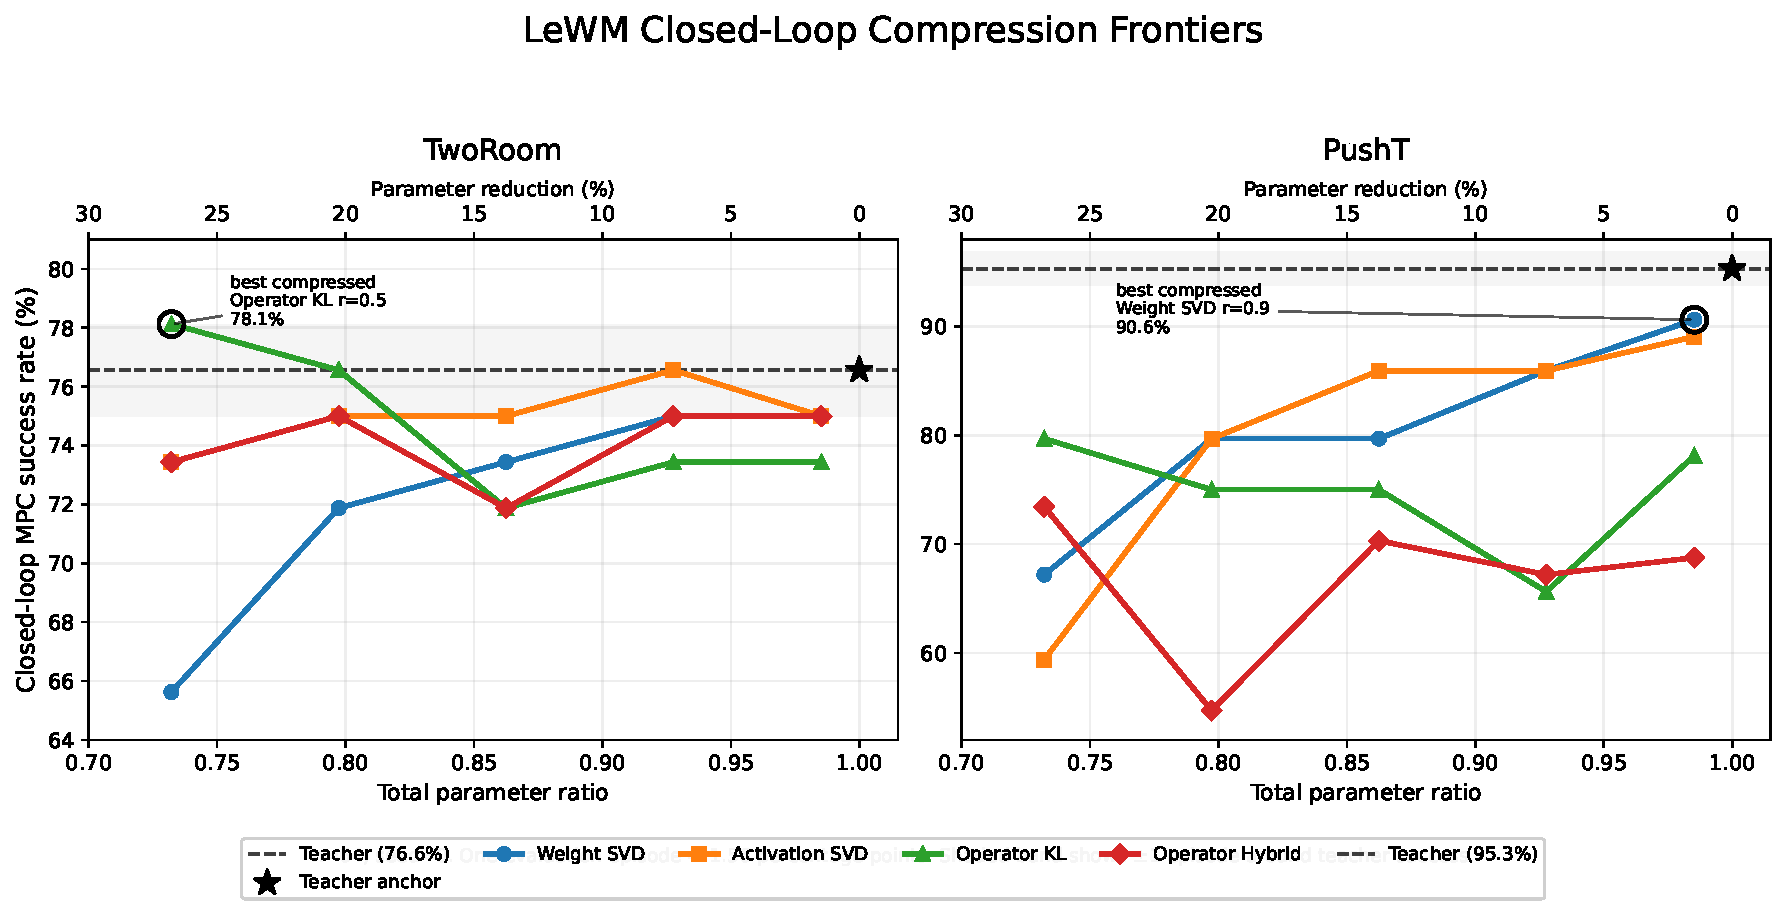
\includegraphics[width=\linewidth]{figures/paper_frontier_lewm_tworoom_pusht_side_by_side.pdf}
    \caption{
    Closed-loop compression frontiers for \textsc{TwoRoom} and \textsc{PushT}.
    Activation-aware SVD provides a strong and stable direct compression baseline, especially on \textsc{TwoRoom}. On \textsc{PushT}, compression is more damaging, and cache-only operator-aware distillation is inconsistent across ranks. These results suggest that planning-aware compression is promising but fragile under limited offline candidate supervision.
    }
    \label{fig:combined-frontiers}
\end{figure}

\subsection{Summary of Observations}
\label{sec:results_summary}

We summarize the main observations as follows.

First, closed-loop performance is not perfectly monotone in compression ratio at \(n=64\). Some lower-rank models outperform nearby higher-rank models by one or two episodes. Because each episode changes success rate by \(1.5625\) percentage points, these local irregularities should be interpreted as evaluation noise unless they persist across additional seeds or larger evaluation sets.

Second, activation-aware SVD is a strong baseline. On \textsc{TwoRoom}, it preserves near-teacher performance even at aggressive compression. On \textsc{PushT}, it is competitive with weight SVD at mild compression and substantially better at \(r=0.7\), though it degrades sharply at \(r=0.5\).

Third, \textsc{PushT} is more sensitive to compression than \textsc{TwoRoom}. The teacher starts at a much higher success rate on \textsc{PushT}, and compression produces larger absolute drops in performance. This suggests that contact-rich manipulation places stricter demands on the fidelity of the compressed predictor.

Fourth, operator-aware fine-tuning is fragile in the current implementation. Although it is motivated by the planning role of the model, matching cached teacher costs does not reliably improve closed-loop MPC success. In many cases, especially on \textsc{PushT}, operator-aware fine-tuning underperforms the compressed initialization.

Finally, offline distillation loss is not reliably predictive of closed-loop performance. Several distilled models reduce or stabilize their cache-based objectives while producing worse MPC success. This indicates a mismatch between the offline candidate distribution used for distillation and the online candidate distribution induced by CEM during closed-loop planning. As a result, future operator-aware methods should either construct caches closer to the planner's test-time distribution or explicitly validate distillation objectives against closed-loop behavior.
% ------------------------------------------------------------
% 7. Analysis
% ------------------------------------------------------------
\section{Analysis}
\label{sec:analysis}

The results above suggest a useful distinction between two kinds of compression objectives. Direct low-rank compression tries to preserve the internal computation of the model, while operator-aware distillation tries to preserve the planner-facing cost function induced by the model. In principle, the second objective is more aligned with how the model is used at test time. In practice, our experiments show that this alignment is fragile: the particular offline operator supervision used here does not always match the distribution of action sequences encountered by the closed-loop planner.

\subsection{Activation-Aware Compression Is a Strong Baseline}
\label{sec:activation_svd_analysis}

Activation-aware SVD is strong because it compresses the predictor while explicitly preserving the linear maps on activations that actually occur under the model's operating distribution. For a predictor layer with weight matrix \(W\), ordinary weight SVD approximates \(W\) directly, independent of which input directions the model uses. In contrast, activation-aware compression approximates the layer output
\[
    XW,
\]
where \(X\) denotes a matrix of calibration activations collected from the model. The relevant approximation problem is therefore not only whether \(W\) is close to a low-rank factorization, but whether the compressed layer produces similar outputs on the activations induced by realistic states, goals, and candidate action sequences.

This is particularly well matched to MPC evaluation. During planning, the cost assigned to an action sequence depends on repeated predictor applications in latent space. If compression preserves the predictor's intermediate activations on the types of inputs produced during planning, then the induced rollout costs are more likely to remain stable. Activation-aware SVD therefore provides a local, behavior-preserving approximation to the predictor without requiring a separate teacher-labeling procedure.

A second advantage is that activation-aware SVD does not depend on imperfect action-candidate labels. It does not ask which sampled action sequence is best, nor does it require a soft distribution over uniformly sampled candidates. Instead, it preserves the computations of the already-trained model on representative inputs. This makes it less vulnerable to overfitting the finite operator cache or to learning spurious distinctions among action sequences that are irrelevant to the planner.

This helps explain why activation-aware SVD is competitive across both environments. On \textsc{TwoRoom}, it preserves teacher-level performance across much of the rank sweep. On \textsc{PushT}, it remains strong at moderate compression, especially around \(r=0.7\), where it substantially outperforms weight SVD. These results suggest that much of the predictor's useful behavior can be preserved by matching activation-space behavior directly.

\subsection{Why Forward KL Can Hurt}
\label{sec:forward_kl_analysis}

The forward KL objective used in our cost-distillation baseline is
\[
    \mathcal{L}_{\mathrm{FKL}}
    =
    \frac{1}{|B|}
    \sum_{s \in B}
    \mathrm{KL}
    \left(
        p_T(\cdot \mid s)
        \,\|\, 
        p_S(\cdot \mid s)
    \right),
\]
where
\[
    p_T(i \mid s)
    =
    \frac{\exp(-\widetilde{c}^{T}_{s,i}/\tau)}
    {\sum_j \exp(-\widetilde{c}^{T}_{s,j}/\tau)},
    \qquad
    p_S(i \mid s)
    =
    \frac{\exp(-\widetilde{c}^{S}_{s,i}/\tau)}
    {\sum_j \exp(-\widetilde{c}^{S}_{s,j}/\tau)}.
\]
Here \(\widetilde{c}^{T}_{s,i}\) and \(\widetilde{c}^{S}_{s,i}\) are normalized teacher and student costs for candidate action sequence \(i\) at state \(s\).

The motivation is reasonable: if the compressed model induces the same cost distribution as the teacher over candidate action sequences, then the planner should make similar choices. However, this assumes that the candidate distribution used during distillation is close to the candidate distribution encountered during planning. In our current setup, the operator cache uses uniformly sampled action sequences in \([-1,1]\). These samples include many poor or irrelevant candidates that the planner would quickly discard during CEM refinement.

Forward KL encourages the student to cover the entire teacher distribution over these candidates. This can be harmful when most candidates are not decision-relevant. Rather than focusing only on preserving the ordering among plausible low-cost plans, the loss also spends gradient budget matching soft probabilities over mediocre or bad candidates. With z-scored costs, the distribution is normalized separately within each state and candidate batch, so relative differences among uniformly sampled candidates can be amplified even when the absolute planning relevance of those candidates is limited.

This creates a possible mechanism for degradation. The compressed initialization may already preserve useful predictor behavior, especially after SVD. Fine-tuning with forward KL can then move the predictor away from this activation-preserving solution in order to better match teacher probabilities on the cache. If the cache distribution is not planner-aligned, lower offline KL need not imply better MPC behavior. This is consistent with our results: cost-KL distillation sometimes improves aggressive compression, but often hurts mild and moderate compression where the compressed initialization was already strong.

\subsection{Why the Hybrid Objective Can Be Unstable}
\label{sec:hybrid_instability_analysis}

The hybrid objective combines the forward KL term with an elite classification loss:
\[
    \mathcal{L}_{\mathrm{hybrid}}
    =
    \lambda_{\mathrm{KL}}
    \mathcal{L}_{\mathrm{FKL}}
    +
    \lambda_{\mathrm{elite}}
    \mathcal{L}_{\mathrm{elite}}.
\]
For each state, the elite set \(E_s\) is defined as the top-\(k\) candidates with lowest teacher cost:
\[
    E_s
    =
    \operatorname{TopK}_{\mathrm{lowest}}
    \left(
        \{c^{T}_{s,i}\}_{i=1}^{C}
    \right).
\]
The student then receives a binary label
\[
    y_{s,i}
    =
    \mathbf{1}[i \in E_s],
\]
and is trained to assign high score to elite candidates and low score to non-elites.

This objective is more directly planner-like than full-distribution KL, since CEM also emphasizes low-cost elites. However, it introduces a different source of instability. The top-\(k\) boundary can be noisy. If the \(k\)-th and \((k+1)\)-th candidates have nearly identical teacher costs, then the binary label changes sharply even though the underlying teacher preference is weak. In that case, the elite classification loss can impose hard distinctions between candidates that are effectively tied.

Balanced BCE can further amplify this issue. Since there are many more non-elite candidates than elite candidates, the balanced loss upweights the relatively small positive elite set. This is useful when elite labels are reliable, but risky when the elite boundary is unstable. A small number of noisy positives can exert a large gradient on the predictor.

The KL and elite terms may also create conflicting pressures. The KL term asks the student to match a soft cost distribution over all sampled candidates, while the elite term asks for a sharper binary separation between top-\(k\) and non-top-\(k\) candidates. If the teacher distribution is soft because many candidates are near-tied, but the elite BCE imposes hard labels, then the two losses are not fully aligned. This may explain why the hybrid objective often performs worse than both the direct SVD initialization and the KL-only objective, especially on \textsc{PushT}.

Importantly, this does not mean that planner-aware supervision is a bad idea. Rather, it suggests that the particular hybrid loss used here is too sensitive to finite candidate sampling and top-\(k\) label noise. A more robust version may need margin-aware labels, pairwise preferences with confidence weighting, CEM-refined candidates, or a held-out closed-loop validation signal.

\subsection{Uniform Candidate Caches versus Planner-Aligned Supervision}
\label{sec:uniform_cache_analysis}

The largest limitation of the current operator-aware distillation setup is that the cache is built from uniformly sampled action sequences. For each cached state, the candidate tensor has shape
\[
    \texttt{candidate\_actions}
    \in
    \mathbb{R}^{S \times C \times H \times A},
\]
with \(S=512\) states, \(C=128\) candidates, horizon \(H=5\), and action dimension \(A\) depending on the environment. These candidates are sampled uniformly rather than generated by the CEM planner.

At test time, however, the planner does not rely on a fixed uniform candidate distribution. CEM begins with broad samples, evaluates them, selects elites, and repeatedly updates the sampling distribution toward lower-cost regions. The action sequences that determine the final executed action are therefore not uniformly distributed. They are biased toward the model's own low-cost regions after several rounds of optimization.

This creates a train-test mismatch for operator distillation. The student is trained to match teacher costs over uniformly sampled candidates, but evaluated inside a planner whose later candidates are CEM-refined. In other words, the cache supervises the cost landscape globally or semi-globally, while the controller depends on local ranking quality near the planner's elite regions.

This weakens the operator-aware claim. Strictly speaking, our current methods are not matching the teacher's online planning operator. They are matching a cached approximation to the teacher's cost function under a uniform candidate proposal distribution. That approximation can still be useful, especially at aggressive compression where the predictor has lost substantial structure. But it is not guaranteed to preserve the decisions made by MPC.

A more planner-aligned protocol would include candidate sequences produced by the teacher's CEM process, such as initial random candidates, intermediate CEM elites, final elite candidates, and the chosen action sequence. Distillation could then focus on preserving rankings and margins among candidates that the planner actually considers plausible. This would better connect the offline objective to the closed-loop success metric.

\subsection{Noise and Evaluation Resolution}
\label{sec:evaluation_noise_analysis}

The current results are preliminary because each model is evaluated on \(n=64\) episodes with a single seed. At this evaluation size, one episode corresponds to
\[
    \frac{1}{64} \times 100 = 1.5625
\]
percentage points. Therefore, differences of one or two episodes correspond to \(1.56\) to \(3.13\) percentage points and should not be overinterpreted.

This matters for several apparent improvements. For example, an operator-distilled model that exceeds the teacher by one episode in a single run is not necessarily better than the teacher. It may simply have succeeded on a slightly different subset of sampled evaluation episodes or benefited from stochasticity in CEM. Similarly, small rank-to-rank non-monotonicities do not necessarily indicate a meaningful compression effect.

The strongest conclusions are therefore qualitative and pattern-based rather than based on isolated point comparisons. The reliable patterns are: direct SVD baselines are strong, activation-aware compression is especially stable on \textsc{TwoRoom}, \textsc{PushT} is more sensitive to compression, and cache-only operator-aware fine-tuning is inconsistent. More definitive claims would require larger evaluation sets, multiple random seeds, and ideally confidence intervals or paired episode-level comparisons.

For this reason, we frame the present study as an empirical stress test of operator-aware compression for latent world models rather than as a final benchmark. The results identify a real failure mode: minimizing an offline operator loss does not necessarily improve closed-loop planning. This failure mode is itself informative, because it clarifies what future planning-aware compression methods must control for.

% ------------------------------------------------------------
% 8. Toward Planner-Aligned Operator Distillation
% ------------------------------------------------------------
\section{Toward Planner-Aligned Operator Distillation}
\label{sec:planner_aligned_distillation}

The negative and mixed results from cache-only operator distillation should not be interpreted as evidence against planner-aware compression in general. The original motivation remains sound: if a world model is used through a planner, then the compressed model should ideally preserve the decisions induced by the planner, not merely the weights or intermediate activations of the uncompressed network. A model can have small prediction error while still assigning the wrong relative costs to action sequences, and a small change in cost ordering can change the action selected by MPC. From this perspective, operator-aware compression is a natural objective.

However, our experiments suggest that the current form of operator distillation is not sufficiently aligned with the actual planning process. The cache is built from uniformly sampled action sequences, while closed-loop MPC uses CEM to iteratively concentrate samples around low-cost regions. Therefore, the current distillation objective teaches the student to imitate the teacher on a broad offline action distribution, not necessarily on the action regions that determine the executed control. A more appropriate objective should focus on preserving the teacher's decision structure near planner-relevant candidates, while avoiding unnecessary changes to already good compressed initializations.

In this section, we outline several concrete directions for planner-aligned operator distillation. We view these as natural next experiments rather than claims established by the current results.

\subsection{Top-\(k\) Renormalized KL}
\label{sec:topk_kl}

A first modification is to restrict distribution matching to the teacher's elite candidates. Instead of matching the teacher and student distributions over all uniformly sampled action sequences, we can define a KL objective only over the top-\(k\) candidates under the teacher cost.

For a state \(s\), let the teacher costs over \(C\) candidate action sequences be
\[
    c^T_{s,1}, \ldots, c^T_{s,C},
\]
and let
\[
    E_s
    =
    \operatorname{TopK}_{\mathrm{lowest}}
    \left(
        \{c^T_{s,i}\}_{i=1}^{C}
    \right)
\]
denote the indices of the \(k\) lowest-cost candidates. We then define teacher and student distributions only on this elite set:
\[
    p_T^{(k)}(i \mid s)
    =
    \frac{\exp(-\widetilde{c}^{T}_{s,i}/\tau_T)}
    {\sum_{j \in E_s}\exp(-\widetilde{c}^{T}_{s,j}/\tau_T)},
    \qquad i \in E_s,
\]
and
\[
    p_S^{(k)}(i \mid s)
    =
    \frac{\exp(-\widetilde{c}^{S}_{s,i}/\tau_S)}
    {\sum_{j \in E_s}\exp(-\widetilde{c}^{S}_{s,j}/\tau_S)},
    \qquad i \in E_s.
\]
The top-\(k\) renormalized KL loss is
\[
    \mathcal{L}_{\mathrm{top}k\text{-}\mathrm{KL}}
    =
    \frac{1}{|B|}
    \sum_{s \in B}
    \mathrm{KL}
    \left(
        p_T^{(k)}(\cdot \mid s)
        \,\|\,
        p_S^{(k)}(\cdot \mid s)
    \right).
\]

This objective is closer to the CEM update rule than full forward KL. CEM does not treat all sampled candidates equally; it selects a small elite subset and updates the sampling distribution using those elites. A top-\(k\) KL similarly focuses the learning signal on candidates the teacher considers good. It avoids spending gradient budget on matching the relative probabilities of many poor candidates that would not affect the planner's final action.

This objective is still not fully planner-aligned, because the top-\(k\) set is drawn from uniformly sampled candidates rather than CEM-refined candidates. However, it is a minimal modification of the existing cache-only pipeline. It can reuse the current stored fields \texttt{teacher\_costs}, \texttt{topk\_indices}, and \texttt{candidate\_actions}. It would also fit the current distillation script structure: sample states, sample or retrieve candidates, compute student costs, restrict to teacher top-\(k\), renormalize, and optimize a KL loss.

A reverse version is also plausible:
\[
    \mathcal{L}_{\mathrm{top}k\text{-}\mathrm{RKL}}
    =
    \frac{1}{|B|}
    \sum_{s \in B}
    \mathrm{KL}
    \left(
        p_S^{(k)}(\cdot \mid s)
        \,\|\,
        p_T^{(k)}(\cdot \mid s)
    \right).
\]
Reverse KL is more mode-seeking: it penalizes the student for placing probability mass on candidates that the teacher assigns low probability, but it does not require the student to cover every teacher-supported candidate. This may be better matched to planning, where selecting one good action sequence is often sufficient. The risk is that reverse KL can become too sharp and collapse onto a single candidate when the teacher distribution contains several near-equivalent plans. For this reason, a temperature sweep would be necessary.

\subsection{Pairwise Preference Distillation}
\label{sec:pairwise_preference_distillation}

A second direction is to replace distribution matching with pairwise preference learning. In planning, the absolute scale of the cost is less important than the ordering of candidates. If the teacher prefers candidate \(i\) to candidate \(j\), then the student should preserve that preference:
\[
    c^T_{s,i} < c^T_{s,j}
    \quad \Longrightarrow \quad
    c^S_{s,i} < c^S_{s,j}.
\]
This can be enforced with a pairwise logistic loss. For a sampled pair \((i,j)\), define the teacher cost margin
\[
    \Delta^T_{s,i,j}
    =
    c^T_{s,j} - c^T_{s,i},
\]
so that \(\Delta^T_{s,i,j} > 0\) means the teacher prefers \(i\) over \(j\). Define the corresponding student margin
\[
    \Delta^S_{s,i,j}
    =
    c^S_{s,j} - c^S_{s,i}.
\]
A simple preference objective is
\[
    \mathcal{L}_{\mathrm{pref}}
    =
    \frac{1}{|\mathcal{P}|}
    \sum_{(s,i,j)\in\mathcal{P}}
    \log
    \left(
        1 + \exp\left(-\Delta^S_{s,i,j}/\tau\right)
    \right),
\]
where \(\mathcal{P}\) is a set of teacher-preferred pairs. This loss is small when the student assigns lower cost to the teacher-preferred candidate by a sufficient margin.

The key design choice is how to sample pairs. Sampling arbitrary pairs from the uniform candidate set may again waste supervision on trivial comparisons between bad candidates. A more planner-relevant strategy is to compare teacher elites against near-elites:
\[
    i \in E_s,
    \qquad
    j \in N_s,
\]
where \(E_s\) contains the top-\(k\) teacher candidates and \(N_s\) contains candidates near the top-\(k\) boundary, such as ranks \(k+1\) through \(m\). This focuses training on the distinctions most likely to matter for candidate selection.

To reduce sensitivity to near-ties, the loss can be weighted by the teacher margin:
\[
    w_{s,i,j}
    =
    \operatorname{clip}
    \left(
        \frac{\Delta^T_{s,i,j}}{\sigma_s + \epsilon},
        0,
        w_{\max}
    \right),
\]
where \(\sigma_s\) is the within-state standard deviation of teacher costs. The weighted loss becomes
\[
    \mathcal{L}_{\mathrm{wpref}}
    =
    \frac{1}{|\mathcal{P}|}
    \sum_{(s,i,j)\in\mathcal{P}}
    w_{s,i,j}
    \log
    \left(
        1 + \exp\left(-\Delta^S_{s,i,j}/\tau\right)
    \right).
\]
This reduces the effect of ambiguous labels. If the teacher barely distinguishes two candidates, then the student is not strongly penalized for reversing them. If the teacher strongly prefers one candidate, then the student receives a larger gradient.

A margin-ranking version is also possible:
\[
    \mathcal{L}_{\mathrm{margin}}
    =
    \frac{1}{|\mathcal{P}|}
    \sum_{(s,i,j)\in\mathcal{P}}
    \max
    \left(
        0,
        m - \Delta^S_{s,i,j}
    \right),
\]
where \(m>0\) is a target student margin. This objective is easy to interpret, but it introduces a margin hyperparameter and can be brittle if the teacher cost scale varies across states. The logistic preference loss is likely safer because it gives a smooth penalty and can be combined naturally with temperature scaling.

Pairwise preference distillation is attractive because it directly targets the ranking structure used by the planner. It does not require matching the full teacher cost distribution, and it is invariant to additive shifts in the student cost. However, it still depends on the quality of the candidate set. If all candidates are uniformly sampled and far from the planner's eventual solution, then preserving their pairwise ordering may still fail to improve closed-loop control.

\subsection{CEM-Augmented Caches}
\label{sec:cem_augmented_caches}

The most important next step is to change the operator cache itself. Rather than storing only uniformly sampled action sequences, the cache should include candidates generated during the teacher's CEM planning process. This would align the distillation distribution with the action regions that actually determine MPC decisions.

For each cached state \(s\), a CEM-augmented cache could store several candidate groups:
\[
    \mathcal{A}_s
    =
    \mathcal{A}^{\mathrm{init}}_s
    \cup
    \mathcal{A}^{\mathrm{mid}}_s
    \cup
    \mathcal{A}^{\mathrm{elite}}_s
    \cup
    \mathcal{A}^{\mathrm{final}}_s.
\]
Here \(\mathcal{A}^{\mathrm{init}}_s\) contains the initial broad CEM samples, \(\mathcal{A}^{\mathrm{mid}}_s\) contains candidates from intermediate CEM iterations, \(\mathcal{A}^{\mathrm{elite}}_s\) contains elite candidates selected by the teacher, and \(\mathcal{A}^{\mathrm{final}}_s\) contains the final chosen plan or final elite set. The teacher cost is then computed or stored for each candidate:
\[
    c^T_s(a_{1:H})
    =
    \mathcal{C}_T(s, a_{1:H}).
\]

This would support a more faithful planner-aligned objective. For example, one could train on a mixture of uniform and CEM-refined candidates:
\[
    \mathcal{D}_{\mathrm{cache}}
    =
    \alpha \mathcal{D}_{\mathrm{uniform}}
    +
    (1-\alpha)\mathcal{D}_{\mathrm{CEM}},
\]
where \(\alpha\) controls how much global coverage is retained. Uniform candidates help preserve broad cost structure, while CEM candidates focus learning on the decision boundary encountered by the planner.

A CEM-augmented objective could then combine top-\(k\) KL and preference learning:
\[
    \mathcal{L}_{\mathrm{planner}}
    =
    \lambda_{\mathrm{top}k}
    \mathcal{L}_{\mathrm{top}k\text{-}\mathrm{KL}}
    +
    \lambda_{\mathrm{pref}}
    \mathcal{L}_{\mathrm{wpref}}
    +
    \lambda_{\mathrm{TR}}
    \mathcal{L}_{\mathrm{TR}}.
\]
The final term is a trust-region regularizer that prevents distillation from moving too far away from the compressed initialization. If \(\theta_0\) denotes the compressed model parameters before distillation and \(\theta\) the current student parameters, a simple parameter-space version is
\[
    \mathcal{L}_{\mathrm{TR}}
    =
    \|\theta - \theta_0\|_2^2.
\]
A more behaviorally meaningful version would preserve the initial compressed model's costs:
\[
    \mathcal{L}_{\mathrm{TR}}
    =
    \frac{1}{|B|C}
    \sum_{s \in B}
    \sum_{i=1}^{C}
    \left(
        \widetilde{c}^{S}_{s,i}
        -
        \widetilde{c}^{0}_{s,i}
    \right)^2,
\]
where \(c^0\) denotes the cost assigned by the compressed initialization before fine-tuning. This would allow operator distillation to make targeted planner-relevant corrections while discouraging broad degradation of a strong SVD baseline.

From an implementation perspective, CEM-augmented caches are the largest change, but they are also the most scientifically meaningful. The current cache format already stores candidate actions and teacher costs, so the extension does not require changing the core distillation interface. The main addition is a cache-building mode that runs the teacher planner, records candidate sequences from selected CEM iterations, and saves metadata indicating the candidate source. Distillation scripts could then either ignore the metadata or use it to prioritize planner-generated candidates.

The expected outcome is not guaranteed improvement across all settings. If the compressed model already preserves the teacher well, additional fine-tuning may still hurt. But a planner-aligned cache would test the right hypothesis: whether matching the teacher on the action sequences actually considered by MPC improves the closed-loop performance of compressed latent world models. That is a stronger and cleaner experiment than the current cache-only uniform-candidate setup.

% ------------------------------------------------------------
% 9. Limitations
% ------------------------------------------------------------
\section{Limitations}
\label{sec:limitations}

This study is preliminary and should be interpreted as an analysis of compression behavior rather than a definitive benchmark of world model compression methods. The most important limitation is evaluation scale. Our closed-loop results use \(n=64\) evaluation episodes with a single random seed. Since one episode corresponds to
\[
    \frac{1}{64} \times 100 = 1.5625
\]
percentage points, small differences in success rate should not be overinterpreted. Several apparent improvements or degradations may disappear under more evaluation episodes, multiple seeds, or different sampled start-goal pairs.

A second limitation is that we performed limited hyperparameter tuning for the operator-aware distillation methods. We used a fixed training setup across environments and compression levels: \(1000\) distillation steps, \(16\) states per batch, \(64\) candidates per state, AdamW with learning rate \(10^{-4}\), and no weight decay. These settings were chosen to keep the sweep computationally feasible, but they are unlikely to be optimal. In particular, operator-aware fine-tuning may require smaller learning rates, early stopping, trust-region regularization, or environment-specific temperatures.

The operator cache is also limited. Candidate action sequences are uniformly sampled in \([-1,1]\), rather than sampled from the candidate distribution encountered during CEM planning. This means that the distillation objective is not directly matched to the closed-loop planner distribution. The student is trained to imitate teacher costs over random candidate plans, while the deployed planner repeatedly refines candidates toward low-cost regions. This mismatch may explain why reducing the offline distillation loss does not reliably improve closed-loop success.

In the current default runner, validation also uses the training cache unless an explicit held-out cache is provided. Therefore, the validation loss measures fit to the cached operator supervision, not generalization to unseen states or unseen candidate distributions. This limits how much we can infer from the reported distillation losses. A stronger protocol would build separate train and evaluation caches using disjoint state samples and possibly different candidate generation procedures.

Our compression scope is also narrow. We compress only predictor parameters, leaving the encoder and other components untouched. This is a reasonable first step because the predictor is central to latent rollout and represents a large fraction of the model, but it does not characterize the full compression frontier of LeWM. Compressing the encoder, the predictor, or both may lead to different tradeoffs between representation quality, dynamics prediction, and planning performance.

Finally, the experiments are limited to LeWM checkpoints on TwoRoom and PushT. These environments differ substantially in difficulty, but they do not cover the full range of world-model planning tasks. TwoRoom is a simple low-dimensional navigation environment, while PushT is a more visually and dynamically involved manipulation task. Additional environments, especially longer-horizon or higher-dimensional control problems, are needed before making broad claims about operator-aware compression for latent world models.

Overall, the main limitation is not merely that the experiment set is small, but that the current operator-aware distillation setup is probably not the strongest version of the idea. The results show that naive cache-only operator fine-tuning can be fragile. They do not rule out planner-aligned operator distillation with better candidate sampling, held-out validation, trust-region constraints, or objectives focused more directly on elite action regions.

% ------------------------------------------------------------
% 10. Related Work
% ------------------------------------------------------------
\section{Related Work}
\label{sec:related_work}

\paragraph{World models for planning.}
World models learn predictive models of environment dynamics that can be used for control, planning, or policy learning. Early work emphasized compact latent dynamics models for agents acting in imagination, while later methods developed more scalable latent and generative world models for reinforcement learning and control. In model predictive control settings, the world model remains inside the decision loop at test time: candidate action sequences are rolled out under the learned dynamics model, scored according to a task or goal cost, and optimized before actions are executed. Our work focuses on this deployment regime. Since the model is queried many times during planning, compression can directly reduce planning cost, but compression errors can also be amplified by the optimizer.

\paragraph{Latent world models and JEPAs.}
Joint-Embedding Predictive Architectures learn to predict future representations rather than reconstruct future pixels. This is attractive for control because the latent space can discard irrelevant visual detail while preserving task-relevant structure. LeWorldModel is a recent end-to-end JEPA-style latent world model that trains from pixels using a prediction loss together with SIGReg, an anti-collapse regularizer that encourages Gaussian-distributed embeddings. Our study treats LeWM as the teacher world model and asks whether its predictor can be compressed while preserving closed-loop MPC performance.

\paragraph{Efficient world models.}
Efficiency in world models can be pursued at several levels: reducing visual token counts, using compact latent spaces, shortening planning horizons, improving the planner, or compressing the learned model itself. LeWM is already designed to be relatively compact and efficient compared with foundation-model-based world models. Our work studies a complementary question: given a trained latent world model, can post-training compression further reduce model size while preserving planning performance? This differs from designing a smaller architecture from scratch, because the compressed model must preserve a pretrained teacher's planning behavior.

\paragraph{Model compression and low-rank approximation.}
Low-rank approximation is a classical approach to neural network compression. A weight matrix \(W\) is replaced by a product of lower-rank matrices, reducing parameter count and potentially inference cost. Standard weight SVD compresses layers by approximating \(W\) directly. In our setting, this provides a simple post-training baseline for compressing the LeWM predictor. However, preserving weights in Frobenius norm does not necessarily preserve the layer outputs on the activation distribution induced by planning.

\paragraph{Activation-aware compression.}
Activation-aware methods instead approximate the action of a layer on representative inputs. Rather than minimizing \(\|W-\widehat W\|\), they aim to minimize a quantity like
\[
    \|XW - X\widehat W\|,
\]
where \(X\) is a matrix of observed activations. This can be more relevant than weight-space error when the model only visits a structured subset of the full input space. Our activation-aware SVD baseline follows this principle and is one of the strongest methods in our experiments, especially on TwoRoom. The results suggest that preserving predictor behavior on the model's actual activation distribution is a strong default for world model compression.

\paragraph{Knowledge distillation.}
Knowledge distillation trains a student model to imitate a teacher model, often by matching logits, probabilities, intermediate features, or task outputs. Our operator-aware methods can be interpreted as a form of distillation where the teacher signal is not a class distribution, but a cost function over candidate action sequences. The student is trained to assign similar costs or similar elite rankings to candidate plans. Unlike standard supervised distillation, however, the relevant output is used inside a downstream optimizer. Small errors in cost ordering can change the selected action even when the average cost-matching loss is low.

\paragraph{Preference distillation and ranking objectives.}
Preference-based objectives train a model to preserve relative comparisons rather than absolute values. This is closely related to the planning setting, where the planner primarily needs to know which action sequences are better than others. Pairwise preference losses, margin ranking losses, and DPO-style objectives are therefore natural candidates for future operator-aware compression. In our current experiments, the implemented operator losses use forward KL and a hybrid KL-plus-elite objective. The mixed results motivate more explicitly ranking-based or elite-focused objectives.

\paragraph{Planner-aware and task-aware compression.}
Most generic compression methods optimize reconstruction error in weight, activation, or output space. For deployed agents, however, the relevant object is the decision induced by the model and planner together. Planner-aware compression should preserve the cost landscape in the regions searched by the planner and the action selected after optimization. Our work is positioned as an initial empirical study of this idea for latent world models. The main finding is that task- or operator-aware compression is not automatically better: if the supervision distribution is misaligned with the planner, fine-tuning can degrade closed-loop performance.

% ------------------------------------------------------------
% 11. Conclusion
% ------------------------------------------------------------
\section{Conclusion}
\label{sec:conclusion}

We studied post-training compression of latent world models used for closed-loop planning. Using LeWM checkpoints on TwoRoom and PushT, we evaluated predictor compression across a rank sweep and measured performance using closed-loop MPC success rather than only offline reconstruction or distillation losses. This evaluation choice is central: for world models used inside planners, the relevant question is not only whether the compressed model matches the teacher locally, but whether it preserves the behavior of the planner that depends on the model.

Our results show that simple low-rank compression can be surprisingly competitive. In particular, activation-aware SVD provides a strong and stable baseline, especially in TwoRoom, where it preserves or even matches teacher-level success across aggressive compression levels in the preliminary \(n=64\) evaluation. PushT is more sensitive to compression, but weight SVD and activation-aware SVD still form strong baselines at mild compression.

By contrast, the operator-aware fine-tuning methods tested here are fragile. Forward KL and hybrid KL-plus-elite distillation do not consistently improve over their compressed initializations, and on PushT they often degrade closed-loop performance substantially. This does not invalidate the motivation for operator-aware compression. If a compressed world model is deployed through MPC, then preserving the teacher's induced action preferences remains a natural goal. Rather, the results suggest that naive cache-only distillation over uniformly sampled candidate actions is not sufficiently aligned with the planner's actual decision distribution.

The broader lesson is that world model compression should be evaluated at the level of closed-loop behavior. Offline losses, activation errors, and teacher-cost imitation are useful diagnostics, but they are not guaranteed to predict planning success. Future work should develop planner-aligned operator distillation methods that use CEM-generated candidate distributions, focus supervision on elite or near-elite action regions, and regularize fine-tuning so that it does not destroy strong activation-preserving compressed initializations. Under that framing, this work provides both a preliminary compression frontier and a cautionary result: making compression ``operator-aware'' is promising, but only if the operator supervision matches the planner that will actually use the model.

% ------------------------------------------------------------
% Acknowledgments
% ------------------------------------------------------------
\section*{Acknowledgments}

% Optional.
% Acknowledge course/project context, collaborators, compute resources, and open-source codebases.
% Optional.

% ------------------------------------------------------------
% References
% ------------------------------------------------------------
\bibliographystyle{plain}
\bibliography{references}

% ------------------------------------------------------------
% Appendix
% ------------------------------------------------------------
\appendix

\section{Implementation Details}

% Include exact commands, scripts, and output artifacts.
% Mention:
% scripts/run_full_closed_loop_frontier.py
% scripts/compress_predictor_weight_svd.py
% scripts/compress_predictor_activation_svd.py
% scripts/distill_operator_cost_kl.py
% scripts/distill_operator_hybrid.py
% scripts/benchmark_cost_model.py

\section{Additional Tables}

% Full TwoRoom and PushT tables.

\section{Operator Cache Schema}

% Document keys:
% candidate_actions
% teacher_costs
% topk_indices
% teacher_best_index
% teacher_best_first_action
% etc.

\section{Distillation Objectives}

% More detailed derivations if needed.

\section{Additional Figures}

% Extra plots, per-environment plots, frontier variants.

\end{document}